\subsection{Usefull}
Usually we make the mistake of trying to keep the user as informed as possible and we offer you data that
They do not provide new information, it is redundant. All vain information, that does not make any contribution
The marked objective is also outside of being useful. We do not want the user to be distracted or lost in the middle
 of a complete but complex data pool that does not make any sense for it.

The objective is not to create specialized users in the field, but to provide them with the
information in a way that they can apply to their daily life and thus improve it, show data
technical, difficult to interpret will only make the user avoid them

In complex cases, the concepts that are not of daily use for the users, we can resort information
complementary to your disposition so that the user can be informed about the meaning of the data
represented, this practice will provide the user with a greater mastery of the concept and could be more
sure of your reading of the data, since when we direct the user to official sources of information, where they can
get a real explanation, reinforce the credibility of the representations we are making. In any case,
outside of the main representation, because the user will not have to access this information continuously.

\subsubsection{How to solve it} 
Focus on the objective, show the data directly related to our goal, do not annotate the data
simply because they appear in the data set, and not add technical details irrelevant to the user.

\subsubsection{How we solve it. Aire Guru} 

The data set used contains data such as the indicator of the measurement station, if the station is fixed or mobile
and extra-specific measures for an application that is provided by the same company that collects the data. For our
tool, these data are not useful.
For our tool only the coordinates where the measurement station is located have been used, the moment in
which was the measure and the most relevant value of the five pollutants Co, No2, O3, Pm1, Pm 2.5 and Pm10.

In addition, the measurement is unique for everyone and the general, the AQI, the ranges are exactly the same for everyone, so the user
you just have to make the effort to understand a single concept.

If the measure does not exist, we will simply ignore it. We do not provide explanations or values such as 0 that can reach
error, as if there was no pollution.


In the following figure we see the difference between the zone history and the personalized, the first of them does not show
the point where the measure was taken since it has been selected in the main map. We also like for the history of
zone there is no filter for hours, since the measurements are reported every hour, this means that we will not find
intermediate measures in the data set.
 
\begin{figure}[ht]
    \centering
    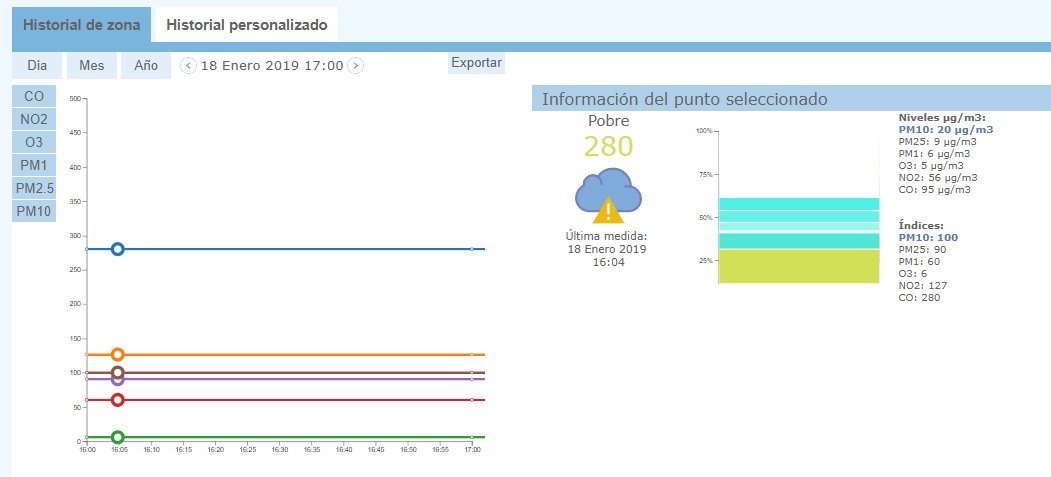
\includegraphics[width=11cm]{zoneRecords}
    \caption{Zone Records}
\end{figure}
\begin{figure}[ht]
    \centering
    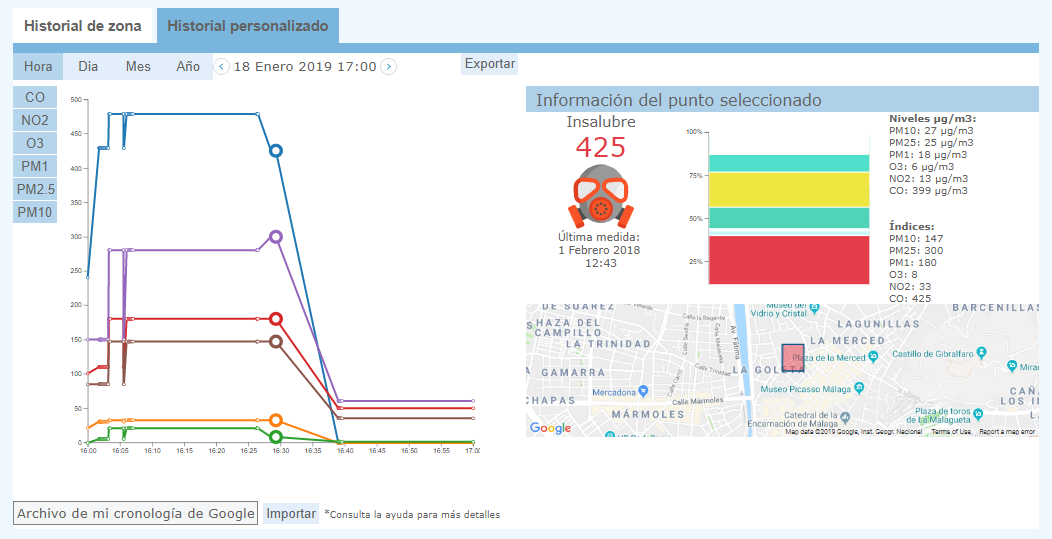
\includegraphics[width=11cm]{personalRecords}
    \caption{Personal Records}
\end{figure}


\elsparagraph{Evaluation}  
\begin{itemize}
    \done The information not relevant to the user has been removed.
         \crossed Exact measurements have been offered. This data is too technical for the user. But nevertheless,
         It contributes truthfulness to the data and has positioned itself in a secondary place so that it does not distract the user.
         \crossed It has implemented a functionality to export the data, the comments of our testers discovered
         that this functionality for the average user is not useful, since they do not have the necessary tools to
         analyze the data and all the information is in the tool represented in a better format.
    
\end{itemize}
 \newpage